%!TEX root = ../BGP_for_networks_who_peer.tex
% chktex-file 44
\chapter{Introduction}
  There are many BGP related trainings out there. Most of them opt for the ``one training for all'' approach.
  This is not the goal of this training. This BGP training is aimed at network engineers working for
  networks who are connected to one or more upstream providers and also participate in peering at an Internet Exchange (IXP).

  Therefore, the focus will be on eBGP, traffic engineering, filtering, and security.

\section{What is BGP?}
Some quick facts about BGP:
\begin{itemize}
  \item BGP is a routing protocol
  \item BGP stands for \textbf{B}order \textbf{G}ateway \textbf{P}rotocol
  \item BGP was first defined in 1989 in \rfc{1105}
  \item Since then, BGP has been continuously extended and updated
  \item The predecessor of BGP was called EGP
    (Exterior Gateway Protocol, defined in 1982, \cite{rfc827})
  \item BGP is standardized. Internet standards are called \glspl{rfc}.
    There is a process for creating and updating them.
    The institution responsible for this is called the \gls{ietf}.
    All \glspl{rfc} are public and can be viewed at \href{https://rfc-editor.org}{https://rfc-editor.org}.
  \item BGP runs on top of TCP - which takes care of reliable transport of BGP messages.
\end{itemize}

\section{Elements of routing}
\subsection{IP prefixes}
One of the key elements in Internet routing is the \emph{prefix}. A prefix is
the network part of an IP address. Prefixes are expressed as follows: The prefix itself, a
slash, and a prefix length. See figure \ref{fig:prefix} for an example for IPv4.
It is important to know, that the host part of an IP prefix contains only zeros.
\begin{figure}
  \centering
  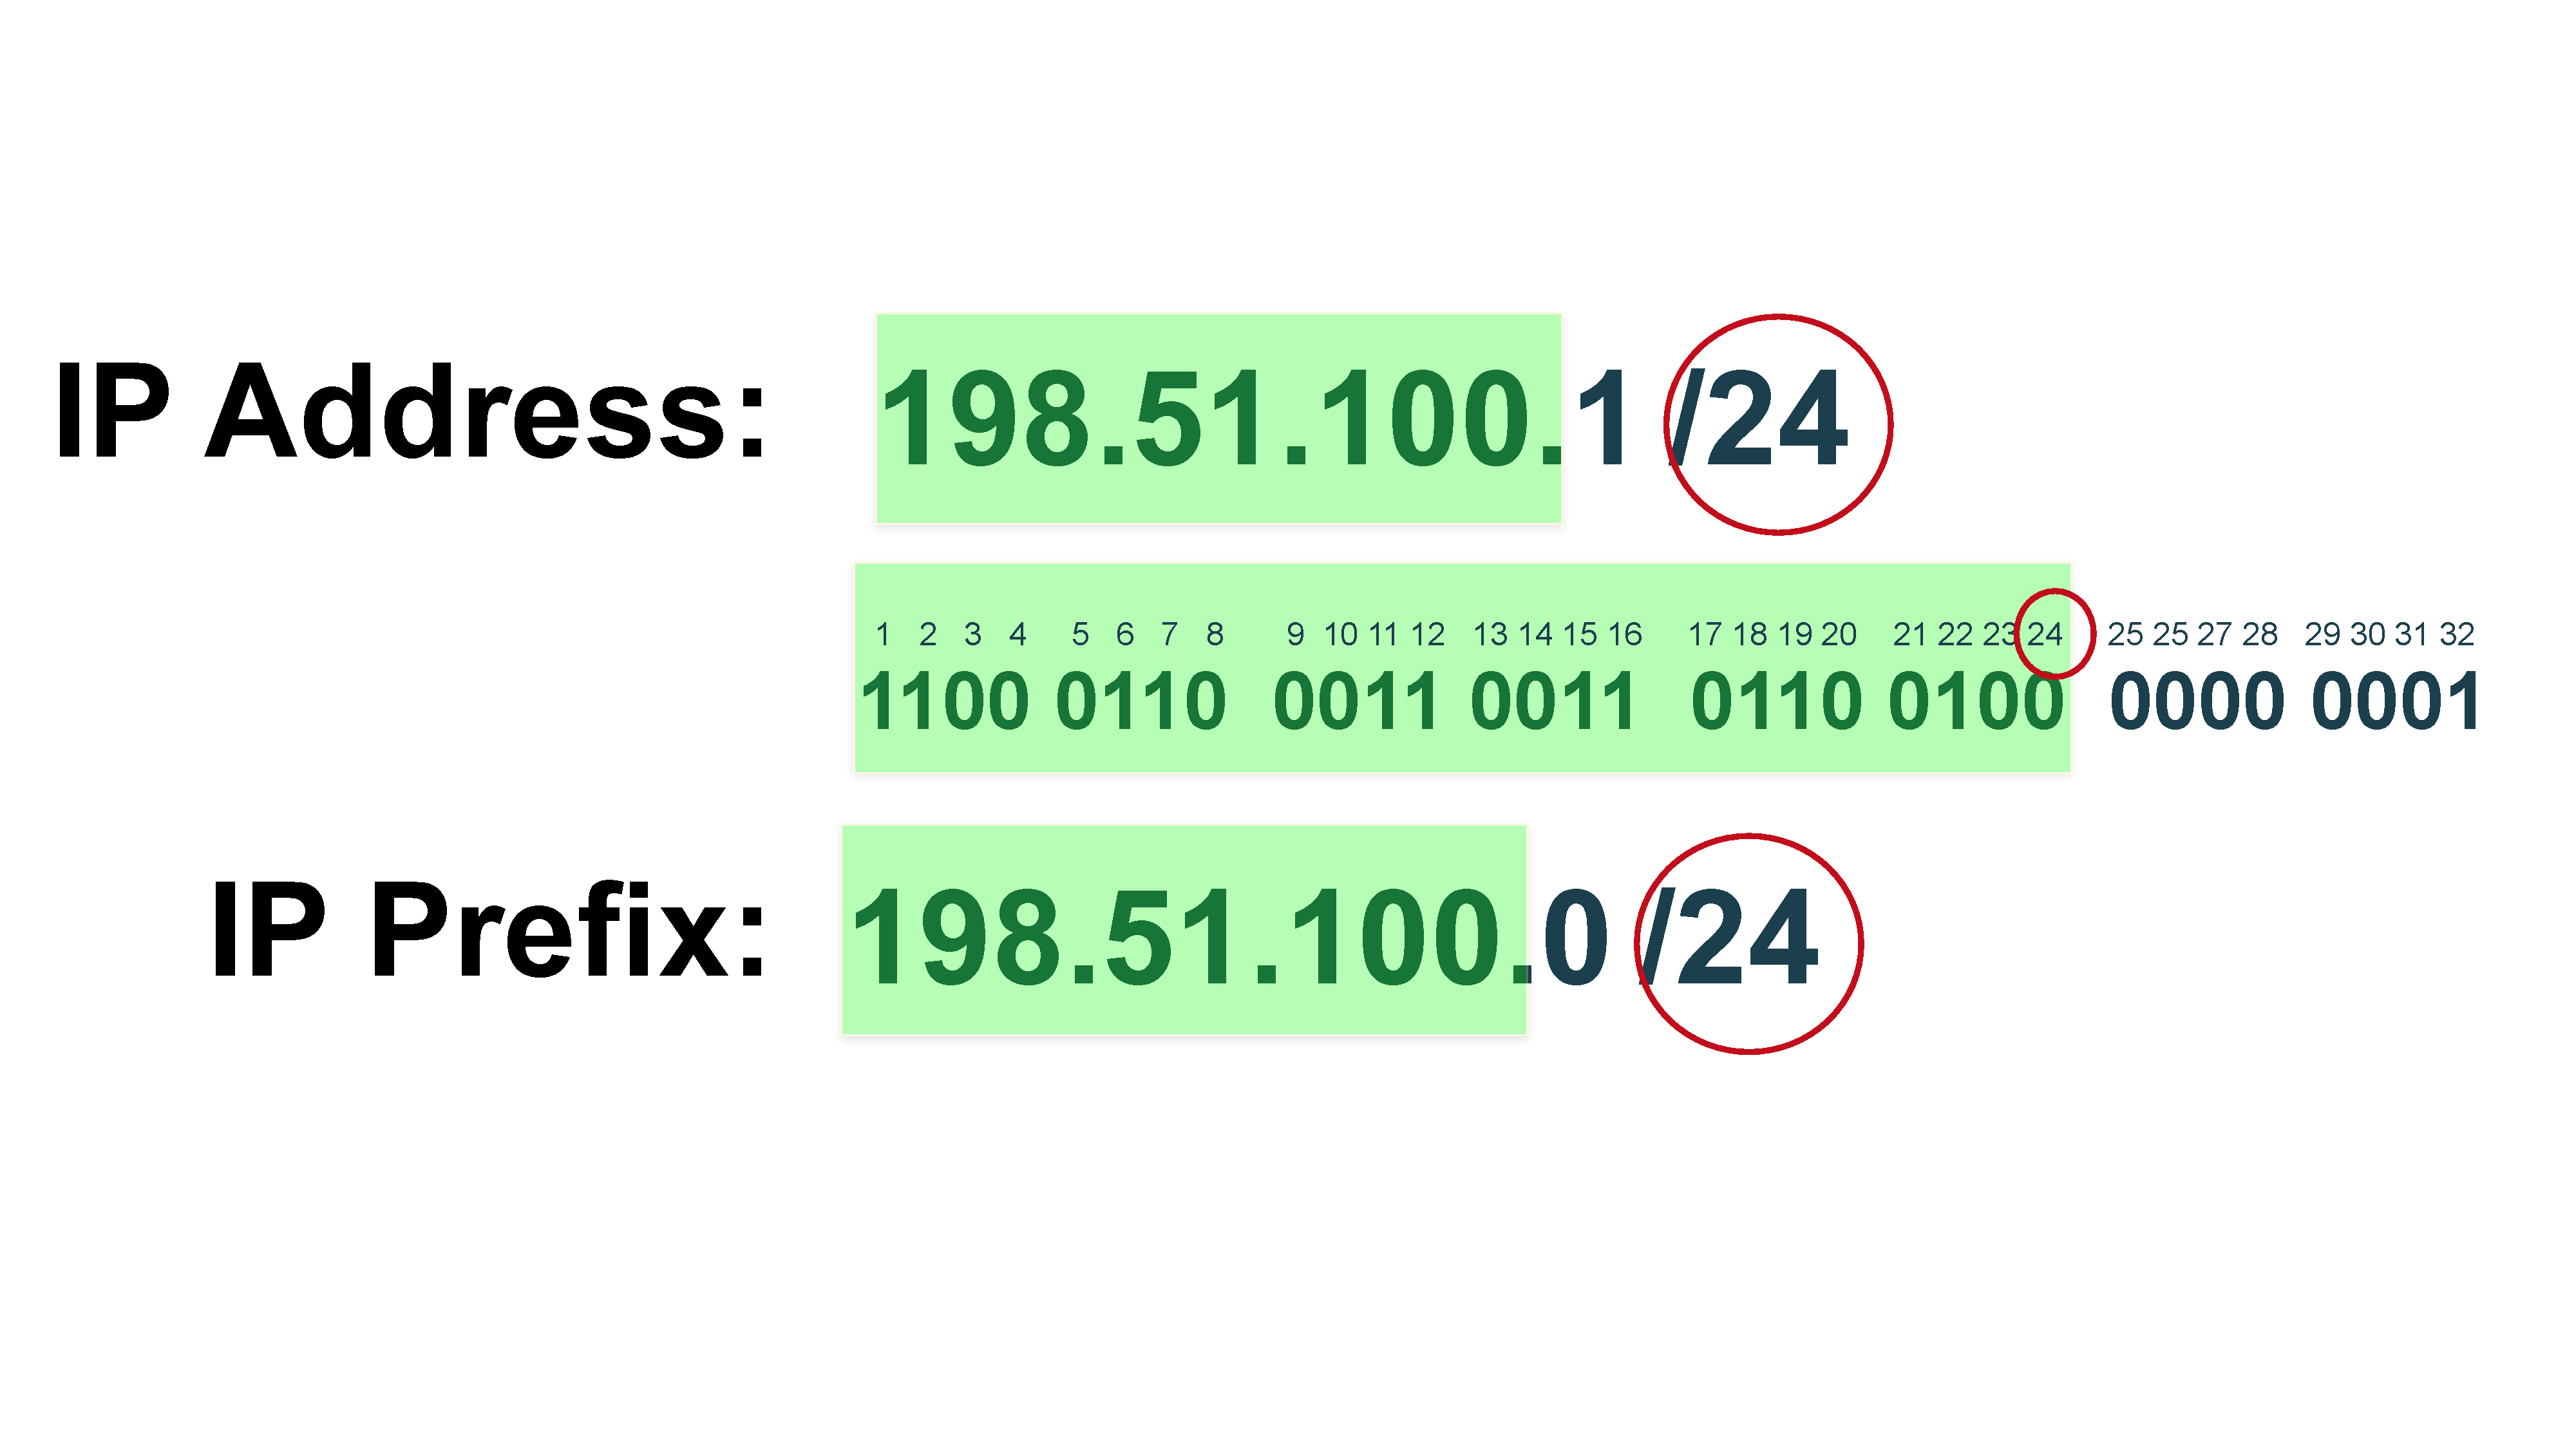
\includegraphics[width=\linewidth,page=1]{img/Drawings.pdf}
  \caption{An IP address and the corresponding IP prefix}
  \label{fig:prefix}
\end{figure}

IPv6 prefixes are similar; they are written as follows: \ip{2001:db8:517::/48}.
Here also the host part is all-zero.

The number behind the `/' is called the prefix length. This is the number of bits
in the network part. The smaller the number, the larger the prefix (larger because
there is more space in the host part of the prefix).

If one prefix is contained in another prefix, you can say that the smaller
prefix (the one with the larger number behind the `/') is \emph{more specific}.

Examples:
\begin{itemize}
  \item \ip{198.51.100.0/26} is more specific than \ip{198.51.100.0/24}.
  \item \ip{2001:db8:6695::/48} is more specific than \ip{2001:db8::/32}.
\end{itemize}

See table~\ref{tab:prefixornot} for some examples of prefixes (and things which are not a prefix).
\begin{table}[hbp]
  \caption{Prefix or not?}
  \label{tab:prefixornot}
  \begin{tabularx}{\textwidth}{lcX}
    \textbf{Item} & \textbf{Prefix?} & \textbf{Explanation} \\
    \hline
    192.168.1.0/24 & Yes & Network part and length \\
    192.168.1.12/24 & No & Host part not zero, this is an IP address and the
                            corresponding netmask \\
    10.0.0.4/30 & Yes & Host part is zero (check!) \\
    80.81.193.0/21 & No & Host part is not zero (convert to binary and check!) \\
    \hline
    2001:db8::/32 & Yes & IPv6 standard prefix \\
    dead:beef:f00d::/48 & Yes & IPv6 is in hexadecimal. So letters a-f are allowed. \\
    2001:db8::4/126 & Yes & Host part is zero. \\
    2001:db8:6695::221:1/96 & No & IPv6 address and netmask. \\
  \end{tabularx}
\end{table}

IPv4 prefixes in the \gls{global routing table} (announced between providers via BGP)
do not come in all sizes. See table \ref{tab:ipv4sizes} for common network sizes. Usually you will not find IPv4 prefixes smaller then /24 in the \gls{global routing table}.
\begin{table}[hbp]
  \caption{Common IPv4 network sizes}
\label{tab:ipv4sizes}
  \begin{tabularx}{\textwidth}{rlrX}
    \textbf{Netmask} & \textbf{Subnet mask} & \textbf{Addresses} & \textbf{Typical use} \\
    \hline
    /8 & 255.0.0.0 & \(2^{24} =\) \tiny{16777216} & Largest block allocated to Internet
        Service Providers (ISPs) or assigned to end users \\
    /9 \ldots /15 \\
    /16 & 255.255.0.0 & 65536 & Large ISP \\
    /17 \ldots /20 \\
    /21 & 255.255.248.0 & 2048 & DE-CIX Frankfurt Peering LAN\\
    /22 & 255.255.252.0 & 1024 & Current allocation of IPv4 space to new ISPs in \gls{RIPE} region \\
    /23 & 255.255.254.0 &  512 \\
    /24 & 255.255.255.0 &  256 & Smallest network routable between providers \\
    /25 & 255.255.255.128 & 128 & \\
    /26 & 255.255.255.192 &  64 & \\
    /27 & 255.255.255.224 &  32 & \\
    /28 & 255.255.255.240 &  16 \\
    /29 & 255.255.255.248 &   8 & Smallest multi-host network (6 hosts)\\
    /30 & 255.255.255.252 &   4 & Often used on point-to-point links (two usable host addresses)\\
    /31 & 255.255.255.254 &   2 & Point-to-point, not possible on all routers\\
    /32 & 255.255.255.255 &   1 & Single host route. Used for loopback interfaces or \gls{blackholing}.\\

  \end{tabularx}
\end{table}

In IPv6 the smallest routable prefix in the \gls{global routing table} is /48. Unlike in IPv4,
when talking about the size of an IPv6 network it is not important how many hosts
an IPv6 network can contain (the standard IPv6 LAN is a /64 and it can
contain
\begin{center}
  \(2^{64} = 18446744073709551616\)
\end{center}
hosts). In IPv6, the question is rather how many /64
sub-networks a network can contain. See table \ref{tab:ipv6sizes} for common IPv6
network sizes.
\begin{table}[hbp]
  \caption{Common IPv6 networks sizes}
  \label{tab:ipv6sizes}
  \begin{tabularx}{\textwidth}{rrXX}
    \textbf{Netmask} & \textbf{Addresses} & \textbf{Used for} & \textbf{Why?}\\
    \hline
    /127 & 2 & Point-to-point \\
    /126 & 4 & Point-to-point \\
    \ldots \\
    /64 & \(2^{64}\) see\footnotemark[1]& LAN & Can address as many
      hosts as you need\\
    \ldots \\
    /56 & \(2^{56}\) & Assigned to residential users & Contains 256 /64 subnets \\
    \ldots \\
    /48 & \(2^{48}\) & Assigned to business users & Contains 65536 /64 subnets \\
    \ldots\\
    /32 & \(2^{32}\) & Current minimum allocation size of IPv6 space to ISPs\\
  \end{tabularx}
\end{table}
\footnotetext[1]{\(2^{24} = 18446744073709551616\)}

\subsection{The Autonomous System}
Another element which needs to be introduced before we can begin with BGP is the
\emph{\gls{Autonomous System}}.

\subsubsection{Motivation}
The Internet is and always has been a ``Network of Networks''. So a big network made up from a lot of small, \emph{independent} networks. Instead of ``independent'' you could also say these part-networks are ``\emph{autonomous}'', so we call them ``\emph{Autonomous Systems}''. And to identify themselves against other part-networks of the Internet, each of them gets an identifier, a so-called \emph{Autonomous System Number}.

\subsubsection{What is an Autonomous System?}
In \cite{rfc1930} an \glsreset{AS}\gls{AS} is defined as follows:
\begin{quotation}
  ``The classic definition of an Autonomous System is a set of routers
      under a single technical administration, using an interior gateway
      protocol (IGP) and common metrics to determine how to route
      packets within the AS, and using an inter-AS routing protocol to
      determine how to route packets to other ASes.''
\end{quotation}

This definition is now replaced by the following more general wording (defined in \cite{rfc1930}):
\begin{quotation}
``An AS is a connected group of one or more IP prefixes run by one
      or more network operators which has a SINGLE and CLEARLY DEFINED
      routing policy.''
\end{quotation}

So the focus is on prefixes and how they are routed:
\begin{itemize}
  \item \emph{\ldots connected\ldots}: An Autonomous System is continuous.
    All entities within are connected with each other.
    \footnote{There are exceptions. AS112 for example is independently operated at multiple locations for DNS reverse resolving of private IP space.}
  \item \emph{\ldots group of one or more IP prefixes\ldots}: This is
    about IP prefixes, not about devices. Routers are not even mentioned.
    All prefixes (or prefix, it can range from one to many) are
    grouped together under an AS and identified by an AS number.
  \item \emph{\ldots run by one or more network operators\ldots}: An AS does
    not have to be run by only one operator if all other conditions
    are matched.
  \item \emph{\ldots SINGLE and CLEARLY DEFINED routing policy\ldots}:
    This is the most important part. Internally and externally all prefixes
    belonging to the same AS are routed the same way. That does not mean
    you cannot adjust the announcement of single prefixes.
\end{itemize}



\subsection{Autonomous System Numbers}
An AS is uniquely identified by an \emph{Autonomous System Number} (ASN). ASNs used to be
16-bit numbers  (defined in \cite{rfc1930}) but some years ago the \gls{IANA} was running out of numbers
to distribute,
so the number space of ASNs has been extended to 32-bit. For this, BGP had to be
extended as well; this was done in \cite{rfc6793}.

Today, AS numbers are 32-bit. You can no longer request a 16-bit number unless
you have a very good reason.

\subsubsection{How to get an AS number}
ASNs are administrated and handed out like IP addresses.
The \gls{IANA} assigns blocks of ASNs to
 \glspl{Regional Internet Registry}; they assign them to \glspl{Local Internet Registry} (= Internet Service Providers), and they hand them out to end users.
To get an AS number you can either:
\begin{itemize}
  \item Become a customer (\gls{Local Internet Registry}) of your local \gls{RIR}, or
  \item ask an existing \gls{Local Internet Registry} to get an ASN for you.
\end{itemize}
The procedures for getting an AS number are different for each region, so please
check online, depending on where you are:
\begin{description}
  \item[Europe, Russia or the Middle East:]
    \url{https://www.ripe.net/publications/docs/ripe-679}
  \item[North Amercia:] \url{https://www.arin.net/resources/request.html#asn}
  \item[South America:] \url{http://www.lacnic.net/1016/2/lacnic/ip-request}
  \item[Asia:] \url{https://www.apnic.net/get-ip/get-ip-addresses-asn/asn-requests/}
  \item[Africa:] \url{https://www.afrinic.net/library/policies/1829-afrinic-consolidated-policy-manual#s7_0}
\end{description}
In general, you must justify your need for an AS number (for example, you want to peer or
have multiple upstream providers).

\subsubsection{Looking up AS numbers}
There are a number of ways you can look up AS numbers.

\paragraph{Whois}
is available on most systems with a command line. Simply type in
\emph{whois AS\emph{nnnn}} and check the output.

\paragraph{PeeringDB}
is an online database of networks who peer. Go to
\url{https://peeringdb.com} and type in the AS number in the search field.

\paragraph{RADB}
mirrors all the databases of the \glspl{RIR}. Just type in the AS number in
the search field.

\paragraph{Regional Internet Registries}
websites can be used also to search for \glspl{ASN}.

\subsection{The AS path}
The AS path is built when announcing prefixes via BGP.
Each AS adds its number to the front of the path. The AS can also be added
multiple times to make an artificially longer AS path. See picture \ref{fig:aspath}
for how an AS path is built by announcing and re-announcing an IP prefix.

\begin{figure}
  \centering
  \includegraphics[width=\linewidth,page=2]{img/Drawings.pdf}
  \caption{How an AS path is built}
  \label{fig:aspath}
\end{figure}


\section{Some theory about routing protocols}
\subsection{Classification of routing protocols}
There are several ways to classify routing protocols:
\begin{itemize}
  \item Static vs. dynamic
  \item Interior protocols vs. exterior protocols
  \item Link state vs. distance vector
\end{itemize}

\subsection{Static vs.\ dynamic routing}
In static routing, you configure all the routing decisions into the routers
statically. So if anything in the network changes, routers have no
way to react and change their routing decisions.

In dynamic routing, routers ``talk'' to each other using a routing protocol
about (for example) the network state and/or reachability of IP addresses. So
in case of a network change, routers can adapt to the new situation.

\subsection{Interior protocols vs.\ exterior protocols}
An \acrfull{IGP} is a protocol which routers under one administrative domain use to communicate with each other about network state and reachability. Examples of \glspl{IGP}
are: \gls{OSPF}, \gls{IS-IS}, \gls{EIGRP}, \gls{RIP}.

Exterior routing protocols are protocols which different administrative entities
use to exchange information. Nowadays, BGP4 is the only exterior protocol
remaining.

\subsection{Link state vs.\ distance vector protocols}
In a link state protocol, each router has a map of the whole network and calculates
the best path to a destination. Examples for link state protocols are OSPF and IS-IS.

In a distance vector protocol, the calculation of the best path is done by routers exchanging
the routing tables with each other and choosing the path with the least number
of hops (or in the instance of BGP:\ number of Autonomous Systems) to cross.

Examples of distance vector protocols are \gls{RIP} and \gls{BGP}.

\section{How a router works}
\begin{figure}
  \centering
  \includegraphics[width=\linewidth,page=10]{img/Drawings.pdf}
  \caption{A simplified diagram of a router}
\label{fig:router}
\end{figure}
But how do these different protocols act together in a router? Please see figure \ref{fig:router} - it shows the various tables in a router and how they interact.

\begin{description}
  \item[Forwarding Table] is often realized in hardware (ASICs). It has to be very fast and is consulted for each and every packet a router forwards. How it works and how it is implemented is different for each router.
  \item[Routing Table] exists for each protocol the router is routing (so most of the time, one table for IPv4 and another table for IPv6). Usually for each prefix the router knows about, it contains one next-hop IP address and the interface via which this IP can be reached.
  \item[Static Routes] are simply installed in the routing table.
  \item[Link State Database] is used by OSPF and contains a complete ``picture'' of the network including all nodes and links in between the nodes. OSPF calculates the best path to a destination and installs it as a route (including a next-hop address) in the routing table.
  \item[BGP Prefix Table] contains all received prefixes from all BGP neighbors. After the BGP process has done its \emph{best prefix selection}, \textbf{one} of these routes is installed in the routing table.
\end{description}

\section{BGP and IPv6}
Usually BGP training programs and manuals have their own chapter about IPv6. But as it is now 2018 and IPv6 should be quite common, all information about how to implement IPv6 routing is directly integrated. You should not setup BGP for IPv4 first and add IPv6 capabilities later - best practice is to integrate IPv6 from the beginning.

BGP is much older then IPv6. The first incarnation of BGP was described in \rfc{1105} in 1989 (building on experience with its predecessor protocol \gls{EGP}) - IPv6 was specified in \rfc{1883} in 1995.

BGP4 (the still-current version) and predecessors were built for distributing IPv4 prefixes only. But unlike IP itself and other routing protocols like \gls{OSPF}, BGP4 was designed with extensibility. So it was not necessary to introduce a new protocol; BGP4 was simply extended.

And because nobody wanted to do this over and over again, the extension to BGP4 was not just to accommodate IPv6, but for multiple network protocols. This was published first in \rfc{2283} (but the most current version of the extensions are in \rfc{4760}). The extension was backward compatible, so routers which had them could communicate with routers which did not have them.

\section{Recommendations}
I rarely give recommendations. This book and the corresponding training seminar should give you the knowledge to make your own choices. However, sometimes perhaps an obvious choice migth not be the best one. In this case you might find my recommendations useful, but wether you follow them or not, is up to you.

Recommendations are clearly marked like this:

\fcolorbox{black}{lgray}{
\begin{minipage}{\linewidth}
\dangersign[8ex] \textbf{Recommendation:}
Read, understand, and make your own choice.
\end{minipage}
}
